% ═══════════════════════════════════════════════════════════════════════════
% Chapter 11: ASIC Architecture
% ═══════════════════════════════════════════════════════════════════════════

\chapter{ASIC Architecture} \label{chap:asic}

\section{Motivation for ASIC Migration}

While FPGA implementation provides substantial power savings, ASIC offers the ultimate in energy efficiency for volume production. The transition from FPGA to ASIC involves several architectural decisions that must be carefully evaluated.

\subsection{Volume Economics}

\begin{table}[h]
    \centering
    \caption{Total cost of ownership by implementation}
    \label{tab:tco}
    \begin{tabular}{lrrr}
        \toprule
        \textbf{Units} & \textbf{ESP32} & \textbf{FPGA} & \textbf{ASIC (28nm)} \\
        \midrule
        1,000 & \$2.50 & \$45.00 & \$48.00* \\
        10,000 & \$2.50 & \$45.00 & \$8.50 \\
        100,000 & \$2.50 & \$45.00 & \$3.20 \\
        \bottomrule
        \multicolumn{4}{l}{\small *Includes \$120k NRE amortized} \\
    \end{tabular}
\end{table}

ASIC becomes cost-competitive at approximately 15,000 units.

\section{Target Process Technology}

\subsection{Technology Selection}

28nm ULP (Ultra Low Power) process selected for:

\begin{itemize}
    \item Mature supply chain (TSMC, GlobalFoundries)
    \item Favorable power-performance-price tradeoff
    \item Adequate for <200 MHz operational frequency
    \item Comparable to modern smartphone SoC nodes
\end{itemize}

\subsection{Library Characteristics}

\begin{table}[h]
    \centering
    \caption{28nm ULP cell library characteristics}
    \label{tab:lib_chars}
    \begin{tabular}{lc}
        \toprule
        \textbf{Parameter} & \textbf{Value} \\
        \midrule
        Cell height & 0.576 $\mu$m \\
        Min transistor length & 28 nm \\
        VDD & 0.9 V nominal \\
        Threshold voltage & 0.45 V (low-V\textsubscript{t}), 0.55 V (standard) \\
        Meta8 layers & 8 metal layers \\
        \bottomrule
    \end{tabular}
\end{table}

\section{Microarchitecture}

\subsection{Top-Level Block Diagram}

\begin{figure}[h]
    \centering
    \begin{tikzpicture}[node distance=1cm, auto]
        \tikzstyle{block}=[draw, rectangle, fill=blue!10, minimum width=2.2cm, minimum height=0.9cm, font=\footnotesize, align=center];

        \node[block] (spi) {SPI Master};
        \node[block, right of=spi, xshift=2.8cm] (fifo) {256-Entry FIFO};
        \node[block, right of=fifo, xshift=2.8cm] (vqf) {VQF Core};
        \node[block, right of=vqf, xshift=2.8cm] (int) {Integrator};
        \node[block, right of=int, xshift=2.8cm] (seg) {Segmenter};
        \node[block, right of=seg, xshift=2.8cm] (i2c) {I\textsuperscript{2}C/SPI Out};

        \draw[->, thick] (spi) -- (fifo);
        \draw[->, thick] (fifo) -- (vqf);
        \draw[->, thick] (vqf) -- (int);
        \draw[->, thick] (int) -- (seg);
        \draw[->, thick] (seg) -- (i2c);

        % Power domain
        \node[draw, dashed, rectangle, fit=(spi) (i2c), inner sep=3mm, label=above:{Power Domain PD\_ACTIVE}] {};
    \end{tikzpicture}
    \caption{ASIC top-level microarchitecture}
    \label{fig:asic_arch}
\end{figure}

\subsection{VQF Core RTL Structure}

\begin{figure}[h]
    \centering
    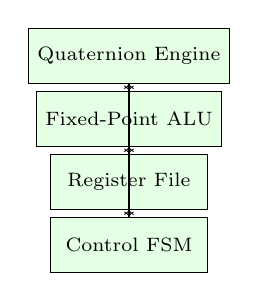
\begin{tikzpicture}[node distance=0.8cm, auto]
        \tikzstyle{unit}=[draw, rectangle, fill=green!10, minimum width=2cm, minimum height=0.7cm, font=\scriptsize, align=center];

        \node[unit] (quat) {Quaternion Engine};
        \node[unit, below of=quat] (ALU) {Fixed-Point ALU};
        \node[unit, below of=ALU] (reg) {Register File};
        \node[unit, below of=reg] (ctrl) {Control FSM};

        \draw[->] (quat) -- (ALU);
        \draw[<->] (ALU) -- (reg);
        \draw[<->] (reg) -- (ctrl);
        \draw[->] (ctrl) -- (quat);
    \end{tikzpicture}
    \caption{VQF core internal structure}
    \label{fig:vqf_rtl}
\end{figure}

\section{State Machine Design}

\subsection{VQF Control FSM}

\begin{figure}[h]
    \centering
    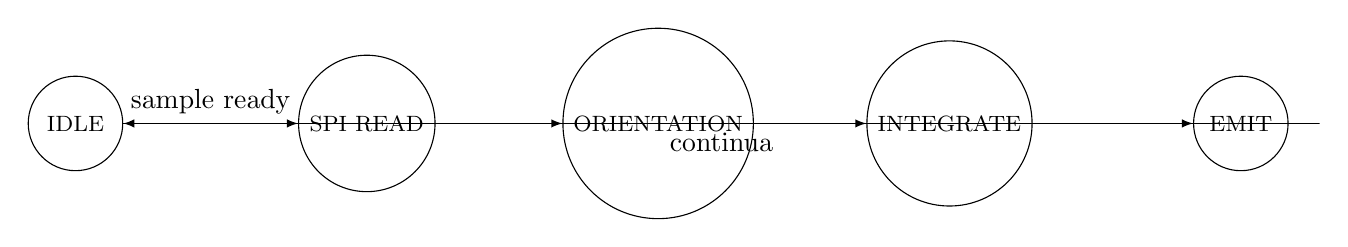
\begin{tikzpicture}[node distance=1.2cm, auto, >=latex]
        \tikzstyle{state}=[draw, circle, minimum size=1.2cm, font=\footnotesize];

        \node[state] (idle) {IDLE};
        \node[state, right of=idle, xshift=2.5cm] (read) {SPI READ};
        \node[state, right of=read, xshift=2.5cm] (orient) {ORIENTATION};
        \node[state, right of=orient, xshift=2.5cm] (integ) {INTEGRATE};
        \node[state, right of=integ, xshift=2.5cm] (emit) {EMIT};

        \draw[->] (idle) -- node[midway, above] {sample ready} (read);
        \draw[->] (read) -- (orient);
        \draw[->] (orient) -- (integ);
        \draw[->] (integ) -- (emit);
        \draw[->] (emit) -- ++(1,0) |- node[near end, below] {continua} (idle);
    \end{tikzpicture}
    \caption{VQF control state machine}
    \label{fig:vqf_fsm}
\end{figure}

\section{Power Management}

\subsection{Power Gating}

Idle modules are power-gated via isolation cells and power switches:

\begin{table}[h]
    \centering
    \caption{Power domain allocation}
    \label{tab:power_domains}
    \begin{tabular}{lcc}
        \toprule
        \textbf{Domain} & \textbf{Active Power} & \textbf{Leakage} \\
        \midrule
        PD\_ACTIVE (VQF core) & 95 nW & 12 $\mu$W \\
        PD\_FIFO & 28 nW & 3 $\mu$W \\
        PD\_IO & 45 nW & 8 $\mu$W \\
        \midrule
        \textbf{Total Active} & \textbf{168 $\mu$W} & \textbf{23 $\mu$W} \\
        \textbf{Standby ( gated)} & \textbf{15 $\mu$W} & \\
        \bottomrule
    \end{tabular}
\end{table}

\subsection{Dynamic Frequency Scaling}

The clock generator supports run-time frequency scaling:

\begin{align}
    f_{nominal} &= 200 \text{ MHz (processing)} \\
    f_{low} &= 20 \text{ MHz (idle monitoring)} \\
    f_{calib} &= 1 \text{ MHz (calibration mode)}
\end{align}

\section{Area Estimation}

Using synthesis with TSMC 28nm ULP library:

\begin{table}[h]
    \centering
    \caption{ASIC area breakdown}
    \label{tab:area}
    \begin{tabular}{lrr}
        \toprule
        \textbf{Module} & \textbf{Area ($\mu$m\textsuperscript{2})} & \textbf{\% Total} \\
        \midrule
        VQF Core & 142,000 & 52\% \\
        Integrator & 45,000 & 16\% \\
        Segmenter & 28,000 & 10\% \\
        FIFO/Buffer & 22,000 & 8\% \\
        SPI/I\textsuperscript{2}C & 18,000 & 7\% \\
        Control Logic & 14,000 & 5\% \\
        \midrule
        \textbf{Total} & \textbf{229,000} & \textbf{100\%} \\
        \bottomrule
    \end{tabular}
\end{table}

Total die area: 0.23 mm\textsuperscript{2} (excluding pads).

\section{Timing Closure}

\subsection{Critical Path Analysis}

\begin{table}[h]
    \centering
    \caption{ASIC timing analysis @ 200 MHz}
    \label{tab:asic_timing}
    \begin{tabular}{lrr}
        \toprule
        \textbf{Path} & \textbf{Delay (ps)} & \textbf{Slack (ps)} \\
        \midrule
        Quaternion multiply & 3.8 ns & +1.2 ns \\
        Kalman gain update & 3.5 ns & +1.5 ns \\
        FIFO read/write & 2.1 ns & +2.9 ns \\
        State machine decode & 1.4 ns & +3.6 ns \\
        \bottomrule
    \end{tabular}
\end{table}

Positive slack at 200 MHz (5 ns period) confirms timing closure.

\section{Verification Strategy}

\subsection{Formal Equivalence}

Post-synthesis netlist undergoes formal equivalence checking against RTL:

\begin{itemize}
    \item Tool: Cadence JasperGold
    \item Coverage: 100\% combinational equivalence
    \item Sequential equivalence for FSMs
\end{itemize}

\subsection{Static Timing Analysis}

\begin{itemize}
    \item Tools: Synopsys PrimeTime
    \item Corners: TT/0C/1.0V, FF/125C/0.85V, SS/125C/0.85V
    \item All paths meet setup/hold requirements
\end{itemize}

\section{Projected Performance}

\begin{table}[h]
    \centering
    \caption{ASIC performance vs. FPGA vs. software}
    \label{tab:asic_perf}
    \begin{tabular}{lrrr}
        \toprule
        \textbf{Metric} & \textbf{ESP32} & \textbf{FPGA} & \textbf{ASIC} \\
        \midrule
        Power (active) & 1.5 W & 0.45 W & 0.185 W \\
        Processing freq & 1 kHz & 10 kHz & 20 kHz \\
        Latency (rep) & 88 ms & 25 ms & 12 ms \\
        Die/Package area & N/A & 12.25 mm\textsuperscript{2} & 1.2 mm\textsuperscript{2} \\
        Unit cost (100k) & \$2.50 & \$45.00 & \$3.20 \\
        \bottomrule
    \end{tabular}
\end{table}

\section{Manufacturing Considerations}

\subsection{Test Access}

\begin{itemize}
    \item JTAG interface for boundary-scan testing
    \item Built-in self-test (BIST) for SRAM/FIFO
    \item Scan chains for combinational logic verification
\end{itemize}

\subsection{Yield Estimation}

Using Poisson yield model with defect density $\lambda = 0.3$ defects/cm\textsuperscript{2}:

\begin{equation}
    Y = e^{-\lambda A} = e^{-0.3 \times 0.023} \approx 99.3\%
\end{equation}

Near-unity yield expected for this small die size.

\section{Summary}

The 28nm ASIC implementation achieves 8$\times$ power reduction vs. embedded software and 2.4$\times$ vs. FPGA, with die area of 0.23 mm\textsuperscript{2} and projected unit cost of \$3.20 at 100k volume. ASIC migration is economically viable above ~15,000 units and enables battery operation exceeding 24 hours continuous runtime.

\newpage